\documentclass{article}
\usepackage{graphicx}
\usepackage{amsmath}
\usepackage{pgfplots}
\usepackage{physics}
\usepackage{cancel}
\usepackage{enumitem}
\usepackage{txfonts}

\pgfplotsset{compat=1.18}

\usepackage[a4paper, top=1cm, bottom=2cm, left=2cm, right=2cm, includehead, includefoot]{geometry}

\begin{document}

\noindent
Physics 4A - Classical Mechanics \hfill Prof. Roger King

\noindent\rule{\textwidth}{0.4pt}

\begin{center}
    \textbf{\LARGE Homework 6} \\
    \vspace{12pt}
    \large Aaron W. Tarajos \\
    \textit{\today}
\end{center}

\noindent\rule{\textwidth}{0.4pt}

\section*{Problem 1}
Two forces $\vec{F_1} = 1.00 \hat i + 2.00 \hat j$ N and $\vec{F_2}$ which is 4.00 N directed at 37$^\circ$, measured from the positive $x$-
axis, act on a 200-g particle. What is its acceleration?

\subsection*{Solution}
Given

\[
	\vec{F}_\text{net} = m \vec{a};
\]
and

\[
	\vec{F}_\text{net} = \left( 1.00\ \hat i + 4\cos 37\ \hat i \right) + \left( 2.00\ \hat j + 4\sin 37\ \hat j \right)
\]
then

\[
	\vec{a} = \frac{\left( 1.00\ \hat i + 4\cos 37\ \hat i \right) + \left( 2.00\ \hat j + 4\sin 37\ \hat j \right)}{0.200} = \boxed{20.973\ \hat i + 22.036\ \hat j\ \text{m}/\text{s}^2}
\]

\section*{Problem 2}
A Saturn V rocket has a mass of $2.70 \times 10^6$ kg and a thrust of $3.30 \times 10^7$ N. What is its initial vertical
acceleration?

\subsection*{Solution}
We can use the same equation but need to consider that the acceleration of gravity is going to decrese the vertical velocity generated by the thrust of the engine.

\[
	\vec{a} = \frac{3.30 \times 10^7 - \left( 2.70 \times 10^6 \cdot 9.81\right)}{2.70 \times 10^6} = \boxed{2.412\ \text{m}/\text{s}^2}
\]


\section*{Problem 3}
What is the reading on the spring scale for each of the situations depicted in the figure below? Each of the
blocks has a mass of 5.00 kg
\begin{figure}[ht]
    \centering
    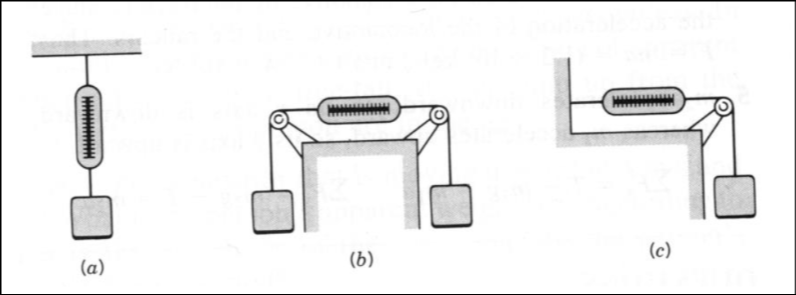
\includegraphics[scale=.3]{drawing-1.png}
\end{figure}

\subsection*{Solution}
\subsubsection*{Part a:}
There are two forces at work, the tension force from the spring and the downward acceleration from gravity. These must sum to zero because the block is at rest;

\[
	T-mg = 0
\]
For the 5.00 kg block, that is

\[
	T = mg \implies 5.00 \cdot 9.81 = 49.05\ \text{N}
\]

\subsubsection*{Part b:}
The tension force from the block on a given side is the same as in part a therefore we have;

\[
	2T - 2(mg) = 0 \implies 5.00 \cdot 9.81 = 49.05\ \text{N}
\]

\subsubsection*{Part c:}
This is no different than part a in terms of the forces, therefore, the reading is;

\[
	T = mg = 5.00 \cdot 9.81 = 49.05\ \text{N}
\]


\section*{Problem 4}
A 7.00-kg block is suspended with two ropes, as shown in the figure. Find the tension in each rope.
\begin{figure}[ht]
    \centering
    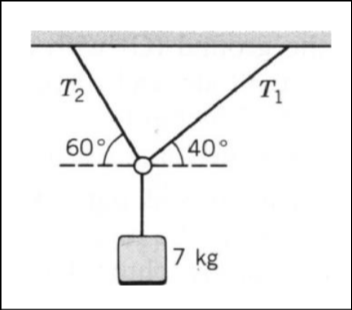
\includegraphics[scale=.4]{drawing-2.png}
\end{figure}

\subsection*{Solution}
Let $T$ be the force of the vertical rope that the block is hanging from. Then;

\begin{equation}
	T_x = 0 \implies T_2 \cos \theta_{T_2} = T_1 \cos \theta_{T_1}
\end{equation}
and

\begin{equation}
	T_y = mg \implies T_2 \sin \theta_{T_2} + T_1 \sin \theta_{T_1}= mg
\end{equation}
Using (1), we obtain

\[
	T_2 = T_1 \frac{\cos \theta_{T_1}}{\cos \theta_{T_2}}
\]
and substituting into (2) we have;

\begin{align*}
	mg &= T_1 \frac{\cos \theta_{T_1}}{\cos \theta_{T_2}} \sin \theta_{T_2} + T_1 \sin \theta_{T_1} \\
	mg &= T_1 \left( \frac{\cos \theta_{T_1}}{\cos \theta_{T_2}} \sin \theta_{T_2} + \sin \theta_{T_1} \right) \\
	T_1 &= \frac{mg}{\left( \frac{\cos \theta_{T_1}}{\cos \theta_{T_2}} \sin \theta_{T_2} + \sin \theta_{T_1} \right)} \\
	T_1 &= \frac{7.0\cdot9.81}{\left(\left(\frac{\cos40}{\cos60}\sin60\right)+\sin40\right)} = \boxed{34.865\ \text{N}}
\end{align*}
then we use $T_1$ to solve for $T_2$ using any of the equations with $T_2$
\[
	T_2 = \left(\frac{7.0\cdot9.81}{\left(\left(\frac{\cos40}{\cos60}\sin60\right)+\sin40\right)}\right)\left(\frac{\cos 40}{\cos 60}\right) = \boxed{53.416\ \text{N}}
\]

\section*{Problem 5}
A painter of mass $M = 75.0$ kg stands on a platform of mass $m = 15.0$ kg. He pulls on a rope that passes
around a pulley, as shown in the figure. Find the tension in the rope given that \\
(a) he is at rest, or \\
(b) he accelerates upward at 0.400 m/s2. \\
(c) If the maximum tension the rope can withstand is 700 N, what happens
when he ties the rope to a hook on the wall?
\begin{figure}[ht]
    \centering
    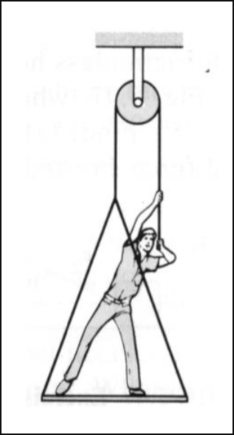
\includegraphics[scale=.4]{drawing-3.png}
\end{figure}

\section*{Solution}
\subsubsection*{Part a:}
Let $T$ represent the tension in the rope. Then

\[
	2T - \left( M + m \right)g = 0
\]
because there is the tension force from the painter to the rope and from the platform to the rope, therefore, the tension is

\[
	T = \frac{\left( 75.0 + 15.0 \right)9.81}{2} = \boxed{441.45\ \text{N}}
\]

\subsubsection*{Part b:}
We add the additional force vector of

\[
	\vec{F}_a = M\vec{a} + m\vec{a}
\]
to the original Tension calculation to obtain
\[
	T = \frac{\left( 75.0 + 15.0 \right)9.81 + \left(75.0 + 15.0\right)0.400}{2} = \boxed{459.45\ \text{N}}
\]

\subsubsection*{Part c:}
If the rope is tied to the wall then there is no longer the second tension force from the painter pulling on the rope, therefore the tension force;

\[
	T = \left( 75.0 + 15.0 \right)9.81 = \boxed{882.9\ \text{N}}
\]
exceeding the maximum load of the rope, so we would expect it to snap.

\section*{Problem 6}
The figure shows a block of mass 1.00 kg is on a frictionless 37.0$^\circ$ incline that is subject to a horizontal force
of 5.00 N.
(a) What is its acceleration? \\
(b) If it is initially moving up the incline at 4.00 m/s, what is its displacement along the incline in 2.10 s?
\begin{figure}[ht]
    \centering
    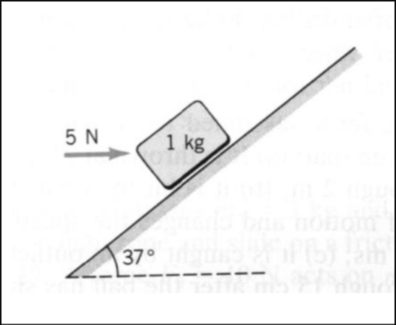
\includegraphics[scale=.4]{drawing-4.png}
\end{figure}

\subsection*{Solution}
\subsubsection*{Part a:}
The force of an object on an incline is given by;

\begin{equation}
	\vec{F}_\text{net} = F_x \cos \theta + F_y \sin \theta
\end{equation}
then, because $\vec{F} = m \vec{a}$

\begin{align*}
	m \vec{a} &= F_x \cos \theta - mg \sin \theta \\
	\vec{a} &= \frac{F_x \cos \theta - mg \sin \theta}{m}
\end{align*}
therefore, the acceleration of the block is;
\[
	\vec{a} = \frac{5 \cos 37 - (1)(9.81) \sin 37}{1} = \boxed{-1.911\ \text{m}/\text{s}^2}
\]

\subsubsection*{Part b:}
Since we are given velocity along the incline, and we solved for acceleration along the incline, we can simply use the one dimensional kinematic equation for constant acceleration. If the dimension of the incline is $r$ then;
\begin{align*}
	\Delta r &= v_0t+\frac{1}{2}at^2 \\
	\Delta r &= (4.00)(2.10)+\frac{1}{2}\left(5 \cos 37 - (1)(9.81) \sin 37\right)(2.10)^2 \\
		 &= \boxed{4.187\ \text{m}}
\end{align*}

\section*{Problem 7}
The two blocks shown in the figure below masses $m_A = 1.95$ kg and $m_B = 3.10$ kg. They are in contact
and slide over a frictionless horizontal surface. A force of 20.0 N acts on B as shown. Find: \\
(a) the acceleration; \\
(b) the force on B due to A; \\
(c) the net force on B; \\
(d) the force on B due to A if the blocks are interchanged.
\begin{figure}[ht]
    \centering
    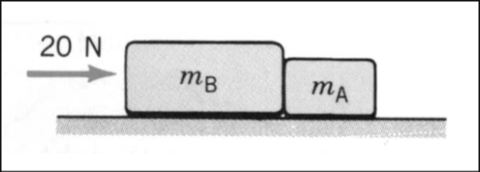
\includegraphics[scale=.4]{drawing-5.png}
\end{figure}

\subsection*{Solution}
\subsubsection*{Part a:}
\[
	\vec{a} = \frac{\vec{F}}{m_B+m_A} = \frac{20}{3.10 + 1.95} = \boxed{3.960\ \text{m}/\text{s}^2}
\]

\subsubsection*{Part b:}
Using Newton's third law we know that the force of $m_A$ on $m_B$ is equal to the force of $m_B$ on $m_A$;
\[
	\vec{F}_{AB} = \vec{F}_{BA}
\]
and
\begin{align*}
	\vec{F}_{AB} &= m \vec{a} \cdot \vec{a} \\
	       &= \left( m_B + m_A \right)\vec{a} \cdot \vec{a} \\
	       &= \left( 3.10 + 1.95 \right)\frac{20}{3.10 + 1.95} \cdot \frac{20}{3.10 + 1.95} \\
	       &= \boxed{79.208\ \text{N}}
\end{align*}

\subsubsection*{Part c:}
\[
	\vec{F}_{\text{net}} = \vec{F} -
\]

\section*{Problem 8}
Two blocks of masses $m_1 = 4.85$ kg and $m_2 = 5.75$ kg kg are on either side of the wedge as shown in
the figure below. Find their acceleration and the tension in the rope. Ignore friction and the pulley.
\begin{figure}[ht]
    \centering
    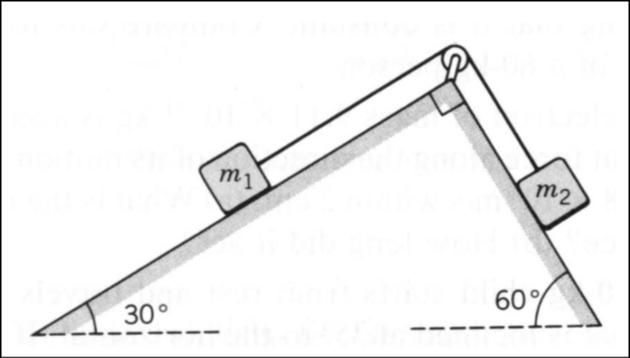
\includegraphics[scale=.4]{drawing-6.png}
\end{figure}

\subsection*{Solution}
We have two blocks to consider the forces for. $m_1$ and $m_2$. For $m_1$ we have Tension less gravity given by;
\[
	\vec{F}_{m1} = T - m_1 g \sin(30)
\]
and for $m_2$ we also have gravity less Tension;
\[
	\vec{F}_{m2} = m_2 g \sin(60) - T
\]
Setting up this problem as a system of equations we have
\begin{align*}
	m_1 \vec{a} &= T - m_1 g \sin(30) \\
	+ \quad m_2 \vec{a} &= m_2 g \sin(60) - T\\
			    \\
	\vec{a}\left(m_1 + m_2\right) &= m_2 g \sin(60) - m_1 g \sin(30) \\
	\vec{a} &= \frac{m_2 g \sin(60) - m_1 g \sin(30)}{(m_1 + m_2)}
\end{align*}
plugging in our values we obtain
\[
	\vec{a} = \frac{5.75 (9.81) \sin(60) - 4.85 (9.81) \sin(30)}{(4.85 + 5.75)} =  \boxed{2.364\ \text{m}/\text{s}^2}
\]
Now we just plugin acceleration to find the Tension
\[
	T = (4.85) (2.364) + (4.85) (9.81) \sin(30) = \boxed{37.432\ \text{N}}
\]

\end{document}
